% deeprl_practice.tex
% Chapter: The Empirics of Deep RL
% What practitioners discover when applying deep RL: the failure modes, their causes,
% and the diagnostic tools that expose them.

I review the empirical pathologies of deep reinforcement learning, their causes, and the diagnostic tools that expose them.

\subsection{The Moving Target Problem}
\label{sec:moving_target}

In supervised learning, the loss function is a \textit{fixed function} of the training data and model parameters. Deep reinforcement learning does not enjoy this property. Each gradient step moves both the current value estimates and the targets simultaneously, creating a ``nonstationary" optimization landscape. The target network heuristic introduced by \citet{mnih2015} slows target drift by periodically freezing a copy of the network, but does not eliminate it. Therefore Bellman residual is a poor proxy for the accuracy of the value function.

\citet{Fujimoto2022} formalize this observation. Let $Q^\pi$ denote the true value function for policy $\pi$, let $\Delta(s,a) = Q(s,a) - Q^\pi(s,a)$ denote the value error, and let $\varepsilon(s,a) = Q(s,a) - (r + \gamma \mathbb{E}_{s',a'}[Q(s',a')])$ denote the Bellman error. Substituting the definition of $Q^\pi$ yields the key identity: $\varepsilon(s,a) = \Delta(s,a) - \gamma \mathbb{E}_{s',a'}[\Delta(s',a')]$. The Bellman error is a \emph{difference} of value errors at consecutive states, not the value error itself. If the errors $\Delta(s,a)$ and $\Delta(s',a')$ are correlated across time (the network is wrong in the same direction at successive state-action pairs), they cancel in the difference and the Bellman error is small regardless of how large the individual errors are.\footnote{In the extreme case, shifting all Q-values by the constant $c/(1-\gamma)$ leaves the Bellman error unchanged at zero while increasing value error by $c/(1-\gamma)$.}

The second failure mode is specific to finite datasets: \citet[Corollary~1]{Fujimoto2022} show that over an incomplete dataset, zero Bellman error is consistent with arbitrarily large value error, because the network can fit unobserved successor pairs to whatever values make the observed residuals vanish.\footnote{The Bellman equation uniquely identifies $Q^\pi$ when enforced over the entire MDP, but over an incomplete dataset it admits infinitely many solutions. Whenever a transition $(s',a')$ that is reachable from the dataset is not itself in the dataset, the network is free to set $Q(s',a')$ at unobserved pairs to whatever value makes the residual vanish on the observed ones, unconstrained by any loss. A network can thus reach near-zero training loss while the value function remains arbitrarily inaccurate over the full state space.}

The dual failure mode appears in policy gradient methods: \citet{IlyasFang2020} find that even when PPO's surrogate objective improves monotonically, episode return can plateau or decline, because the surrogate gradient is poorly aligned with the gradient of the true return.\footnote{\citet{IlyasFang2020} examine the surrogate objective used in Proximal Policy Optimization \citep{Schulman2017}. The PPO clipping mechanism is designed to keep policy updates within a trust region by bounding the probability ratio $\pi_\theta(a|s)/\pi_{\theta_{\text{old}}}(a|s)$. The gradient of the surrogate is poorly aligned with the gradient of the true return, particularly in later training phases where the policy has diverged from the behavior policy used to collect the replay data. The loss metric that practitioners monitor throughout training is measuring something other than what they care about.}

\subsection{The Reproducibility Crisis and Sensitivity to Random Seeds}
\label{sec:reproducibility}

\citet{henderson2018deep} trained five leading policy gradient algorithms (PPO, TRPO, DDPG, TD3, SAC) on six MuJoCo benchmark environments, holding all hyperparameters fixed and varying only the random seed. The resulting learning curves from different seeds were non-overlapping: a seed that performed well under one algorithm performed comparably to a different algorithm's best seeds, making cross-algorithm comparison unreliable.\footnote{Differences as large as 2,000 points in final episode return arose from seed variation alone.} \citet{Agarwal2021} quantify the problem: comparing point estimates from 5 runs per task on Atari 100k yields Type I error exceeding 50\%, meaning a random noise injection appears beneficial in half of all comparisons.

\citet{Agarwal2021} propose the \emph{interquartile mean} (IQM) as a replacement for mean and median when comparing algorithms. The IQM discards the top and bottom 25\% of runs before averaging, reducing sensitivity to outlier seeds. Using these tools and stratified bootstrap confidence intervals, \citet{Agarwal2021} find that several widely-cited algorithmic improvements on Atari 100k vanish or reverse when statistical uncertainty is accounted for.\footnote{They also introduce performance profiles, which plot the fraction of tasks and seeds where an algorithm achieves performance above a threshold $\tau$, as $\tau$ varies from 0 to the maximum. Performance profiles reveal the full shape of the score distribution rather than collapsing it to a single statistic.}\footnote{The fragility extends to hyperparameters. \citet{Eimer2023} conduct a systematic study of hyperparameter sensitivity across 6 algorithms and 17 environments, finding that default hyperparameters from published papers perform competitively in the specific environments used in those papers but generalize poorly across environments. \citet{Patterson2024} synthesize these findings into an empirical design handbook, recommending at minimum 10 seeds per configuration, IQM-based comparisons, and preregistration of hyperparameter search protocols.}

\subsection{Value Overestimation and Spikes}
\label{sec:overestimation}

Q-learning uses the Bellman optimality update
\begin{equation}
    Q(s,a) \leftarrow r + \gamma \max_{a'} Q(s', a'),
    \label{eq:q_update}
\end{equation}
where the maximum is taken over the estimated Q-values of all actions at the successor state. \citet{ThrunSchwartz1993} identify a positive bias intrinsic to this update: if the Q-value estimates contain noise with mean zero, the maximum over noisy estimates is biased upward by Jensen's inequality. An agent that uses a single network for both action selection ($\arg\max$) and value estimation ($\max Q$) systematically overestimates the values of every state it visits, biasing the Bellman target upward at every update step. The bias compounds through bootstrapping: overestimated targets produce overestimated updates, which produce further overestimated targets.

\citet{vanHasselt2010} propose double Q-learning as a remedy: maintain two independent Q-networks $Q_A$ and $Q_B$. Use $Q_A$ to select the greedy action at $s'$, but use $Q_B$ to evaluate that action. Because the two networks are trained on different data, their errors are approximately independent, and the positive bias largely cancels. \citet{vanHasselt2016ddqn} implement this as Double DQN, using the online network for action selection and the periodically-frozen target network for evaluation. On 49 Atari games, Double DQN reduces overestimation by a factor of 3--5 and improves median performance by 20\% relative to DQN.

\citet{fujimoto2018td3} observe that Double DQN's correction is incomplete in continuous-action settings, where the target network and online network remain correlated through shared updates. They propose Clipped Double Q-learning: compute two Q-value estimates $Q_1, Q_2$ with separate networks trained on the same data, and use $y = r + \gamma \min(Q_1(s',a'), Q_2(s',a'))$ as the Bellman target. The minimum operator introduces pessimistic underestimation, which is conservative but avoids the explosive positive bias.\footnote{\citet{Ciosek2019} note that clipped double Q can cause excessive pessimism under high uncertainty, proposing optimistic actor-critic as a counterweight.}

\begin{figure}[t]
\centering
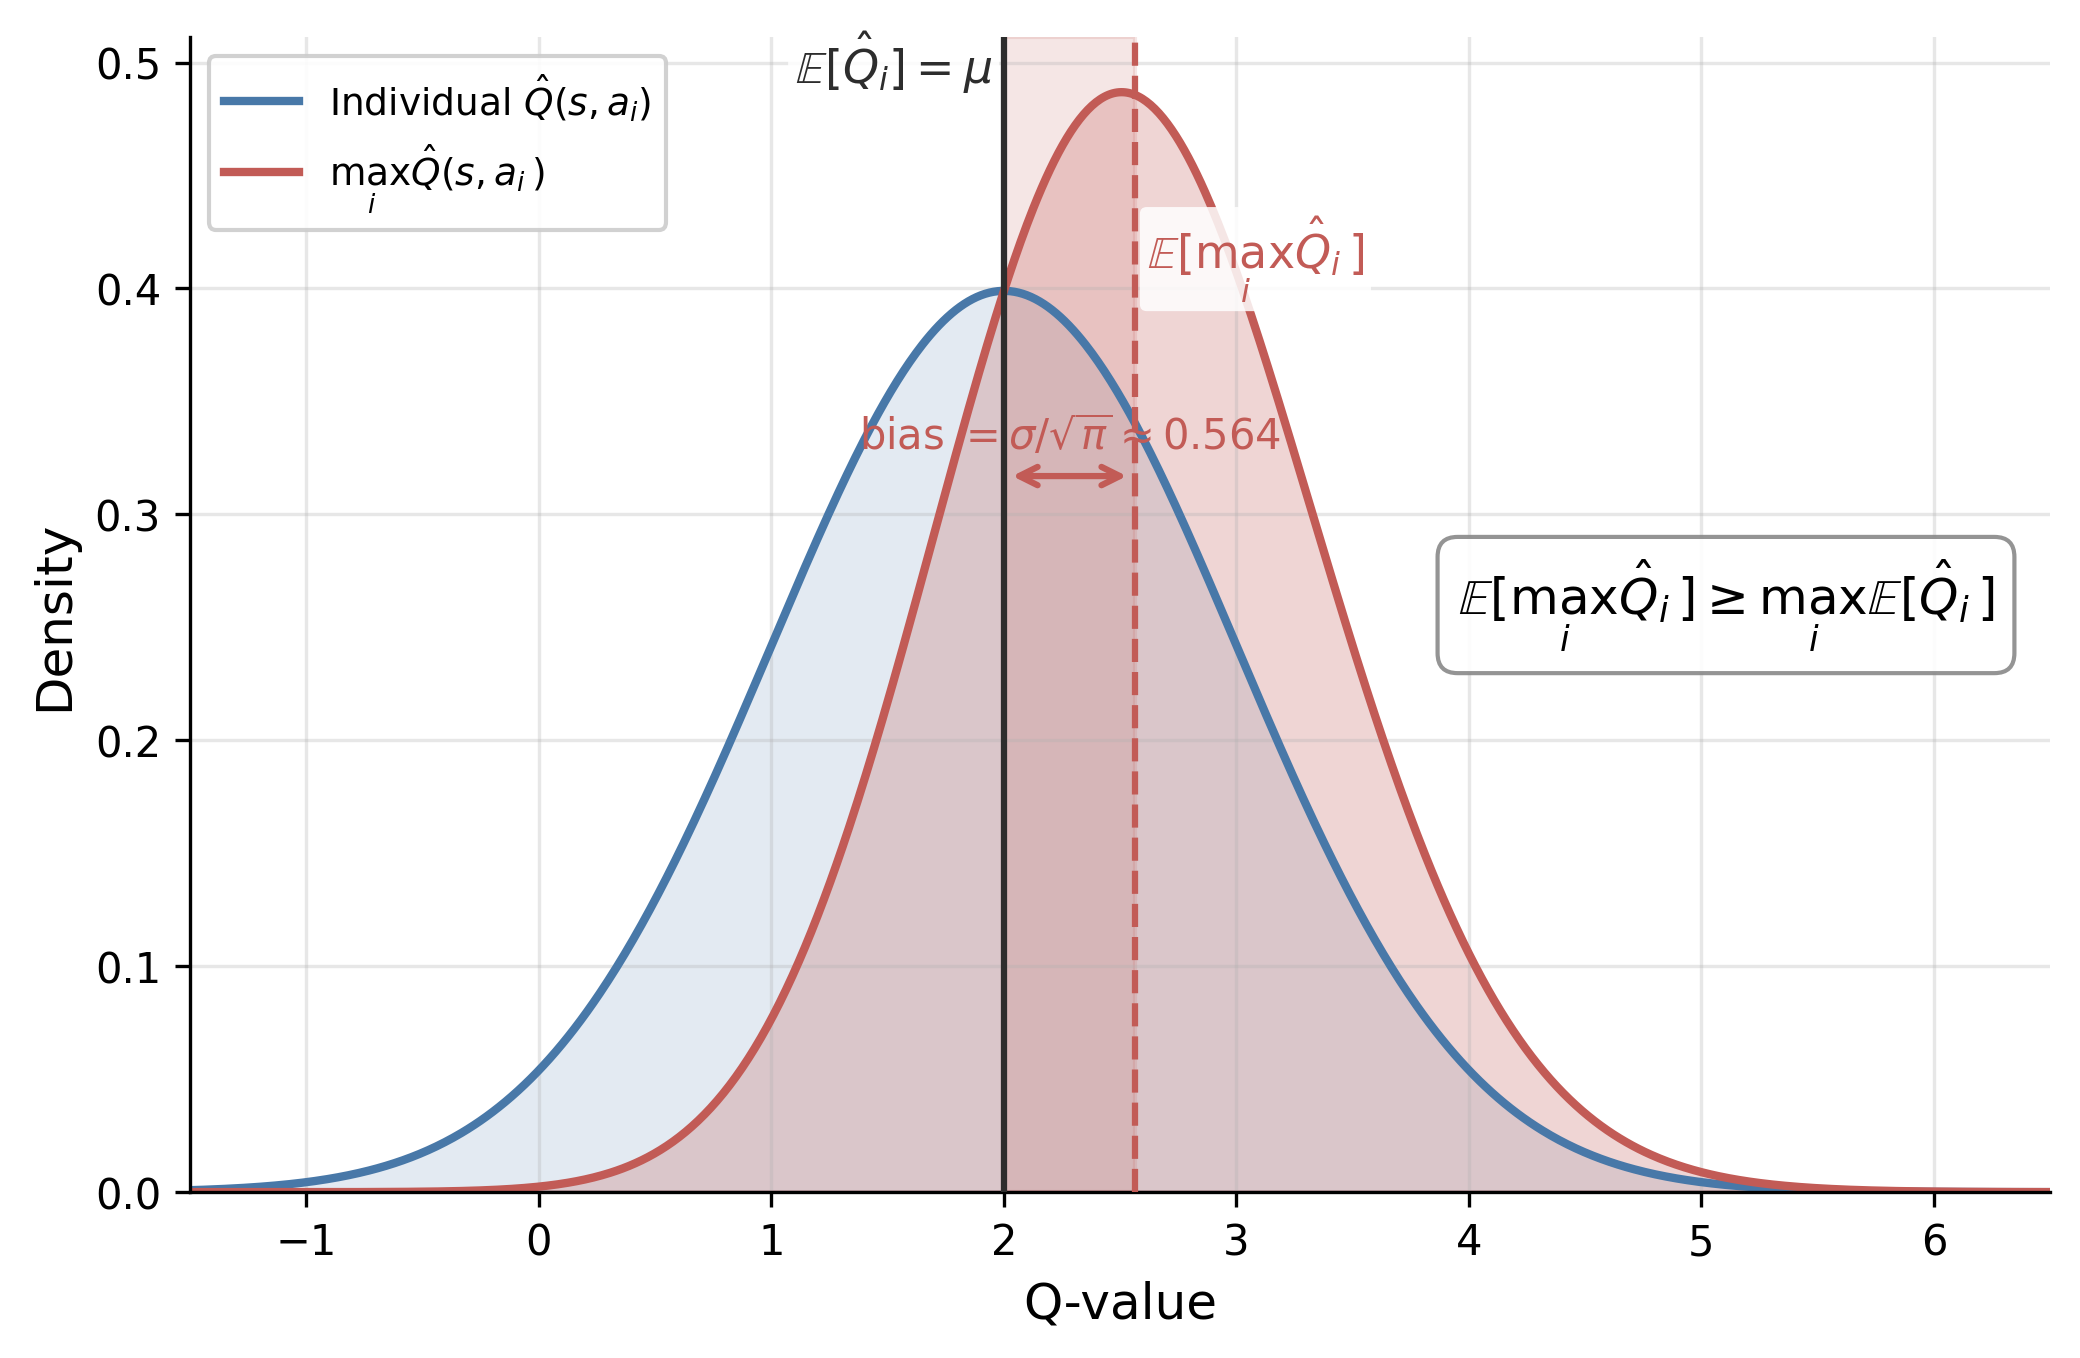
\includegraphics[width=0.7\textwidth]{../ch03b_deeprl_practice/sims/overestimation_bias.png}
\caption{Jensen-inequality illustration of overestimation bias with $n=2$ iid Gaussian Q-estimates. Blue: density of individual $\hat{Q}(s,a_i) \sim \mathcal{N}(\mu,\sigma^2)$. Red: density of $\max_i \hat{Q}(s,a_i)$, shifted right by $\sigma/\sqrt{\pi} \approx 0.56$. The shaded gap is the bias. With $n=100$ actions the bias reaches $2.51\sigma$. Empirical DQN-vs-Double-DQN learning curves are reported in \citet{vanHasselt2010,vanHasselt2016ddqn} and not reproduced here.}
\label{fig:overestimation_bias}
\end{figure}

DQN prevents outright divergence, but \citet{vanHasselt2018} find that \emph{soft divergence} is common. They define it by the realisable range of the value function rather than by any spike criterion: with rewards clipped to $[-1,1]$ and $\gamma = 0.99$, no true value can exceed $1/(1-\gamma) = 100$, so any run whose maximal absolute action value passes 100 has produced an estimate that no policy could justify. Across 336 hyperparameter configurations, 3 replications and 57 Atari games, plain Q-learning soft-diverges on 61\% of runs. The failure is easy to miss, since the estimates typically spike above a million and then settle back below the threshold, and the runs that soft-diverge are the runs that score worse on control. Section~\ref{sec:triad_practice} takes up what reduces this rate and what does not.

\citet{KumarImplicit2021} describe a continuous manifestation of the deadly triad: \emph{implicit under-parameterization}.\footnote{Neural networks trained with bootstrapped TD objectives progressively lose their effective rank, with fewer and fewer neurons contributing distinct directions in the representation. This rank collapse is silent (training loss continues to decrease) but the network's ability to represent new information degrades over time, a form of capacity loss distinct from but related to plasticity loss.}

\subsection{The Deadly Triad in Practice}
\label{sec:triad_practice}

The triad is a property of the composed operator $\Pi_\mu T^\pi$, whose failure to contract is established in Section~\ref{sec:deadly_triad} and made concrete by the divergent star MDP of Theorem~\ref{thm:baird}. No change to the optimizer removes that failure, so the practical question is not which method solves the triad but which methods reduce how often and how badly it bites, and on what evidence. This subsection separates the two kinds of evidence throughout, since the interventions that carry convergence proofs and the interventions that carry measurements are largely disjoint.

Target networks are the primary mitigation and do not eliminate the problem. On the theory side, \citet{zhang2021target} obtain almost sure convergence to a regularized TD fixed point for off-policy linear Q-learning, at the cost of a modified update rule that augments Polyak averaging with two projections and adds ridge regularization, so the guarantee attaches to an algorithm that is not the one practitioners run.\footnote{Their conditions include an ergodic induced chain, linearly independent feature columns, Robbins-Monro step sizes, a bounded feature norm, and projection radii satisfying $R_{B_1} > R_{B_2} > R_{B_1} - \xi > 0$. \citet{chen2022truncation} argue that the ridge term is doing the work by implicitly shrinking the discount factor, so that the problem being solved is no longer the original MDP and the iterates do not reach $Q^*$ even in the tabular case.} \citet{chen2022truncation} show that the target network alone is provably insufficient, exhibiting an MDP on which Q-learning with a target network still diverges, and prove that the target network together with truncation of the value estimate is stable with $\tilde{O}(\epsilon^{-2})$ sample complexity up to function approximation error. \citet{Fellows2023} separate the two step-size regimes and get opposite answers in each. Under diminishing step sizes the asymptotic stability of the update is independent of the refresh period $k$, so temporal difference learning and its target-network variant diverge together, while under step sizes bounded away from zero, the regime practitioners actually use, a finite $k$ exists at which the update contracts to a neighbourhood of the fixed point even where temporal difference learning is unstable. The neighbourhood rather than the point is the price of the fixed step size, since the variance the step size leaves in the updates keeps the iterates off the fixed point and the radius closes only as the step size shrinks.\footnote{Their mechanism is the conditioning of the Jacobian of the temporal difference update, which the target network improves as $k$ grows. On Baird's counterexample they report divergence at $k = 1$, which is ordinary temporal difference learning with a fixed step size, and convergence once $k \geq 500$. An $\ell_2$ regularisation that leaves the temporal difference fixed point unchanged always secures their stability condition; they note that a regularisation which modifies the update instead, as in \citet{zhang2021target}, moves the fixed point.} On the measurement side, target networks are what separates the stable update rules from the unstable ones in \citet{vanHasselt2018}, who also report that applying one to the linear counterexample of \citet{tsitsiklis1997} slows the divergence rather than stopping it.

Experience replay is a sample-efficiency device that pushes against the third leg. Storing transitions from many past policies is what makes the buffer useful and also what makes the updates more off-policy, since the age of the oldest policy in the buffer serves, loosely, as a proxy for how far the data distribution has drifted from the current one \citep{fedus2020revisiting}. Prioritization sharpens the effect in both directions, improving which transitions are replayed and raising the soft-divergence rate from 52\% to 77\% for Q-learning and from 2\% to 23\% for double Q-learning \citep{vanHasselt2018}. Nothing here counteracts the triad, and Section~\ref{sec:replay_reward} records the accompanying finding that a ten-fold larger buffer confers no benefit on DQN at all.\footnote{\citet{fedus2020revisiting} test whether off-policyness explains that null result and reject the explanation, since fixing the age of the oldest policy does not restore the benefit. What does restore it is uncorrected $n$-step returns, without which a Rainbow agent loses 2.3\% median performance when the buffer grows from one million to ten million transitions.}

Multi-step returns dilute the bootstrapping leg by pushing the bootstrap further out, and the measured effect is the largest of any single intervention. One-step Q-learning soft-diverges on 94\% of runs, and at $n = 10$ the rate falls to 21\% \citep{vanHasselt2018}. The Rainbow ablations put multi-step learning and prioritized replay as the two components whose removal costs the most median performance, with the full agent ahead of either ablation on 53 of 57 games \citep{hessel2018rainbow}.

Double Q-learning addresses a different pathology. Its target is the overestimation bias of the max operator (Section~\ref{sec:overestimation}), not the non-contraction of the projected operator, and it reduces divergence only to the extent that inflated targets feed the instability.\footnote{The two are separable in the measurements. Inverse double Q-learning, which uses a separate network to select the bootstrap action but the network being updated to evaluate it, so that it corrects overestimation without bootstrapping on a target network, soft-diverges on 33\% of runs, against 61\% for plain Q-learning and 10\% for double Q-learning \citep{vanHasselt2018}. Within Rainbow the median effect of removing double Q-learning is small, which \citet{hessel2018rainbow} attribute to the distributional support clipping values in a way that already counteracts the bias.}

One result runs against the intuition that the function-approximation leg is worst for the largest models. Soft divergence becomes more frequent as networks grow, from 53\% to 67\% for Q-learning, while the best control performance comes from the largest architectures \citep{vanHasselt2018}. Instability and capacity move together, and the runs that soft-diverge are also the runs that score worse, so the correlation between unrealistic values and poor control is not an artifact of the diagnostic.

Table~\ref{tab:triad_verdict} collects the verdicts.

\begin{table}[t]
\centering
\small
\begin{tabularx}{\textwidth}{@{}>{\raggedright\arraybackslash}p{2.1cm}>{\raggedright\arraybackslash}p{2.5cm}>{\raggedright\arraybackslash}X>{\raggedright\arraybackslash}X>{\raggedright\arraybackslash}p{1.9cm}@{}}
\toprule
Intervention & Leg addressed & Proved & Measured & Verdict \\
\midrule
Target network & Bootstrapping & Convergence to a regularized fixed point under a modified update, linear features \citep{zhang2021target}; stability once truncation is added \citep{chen2022truncation}; no gain from the refresh period under diminishing step sizes, contraction at a finite refresh period under fixed ones \citep{Fellows2023} & Separates stable from unstable update rules; slows but does not stop divergence on the linear counterexample \citep{vanHasselt2018} & Mitigates \\
\addlinespace
Experience replay & Off-policy (worsens) & None & A ten-fold larger buffer gives DQN no gain \citep{fedus2020revisiting} & Not a remedy \\
\addlinespace
Prioritization & Off-policy (worsens) & None & Soft divergence 52\% to 77\% for Q-learning \citep{vanHasselt2018}; one of the two most valuable Rainbow components for performance \citep{hessel2018rainbow} & Not a remedy \\
\addlinespace
Multi-step returns & Bootstrapping & None & Soft divergence 94\% at $n=1$ to 21\% at $n=10$ \citep{vanHasselt2018} & Mitigates \\
\addlinespace
Double Q-learning & Overestimation, not a leg of the triad & None for divergence & 10\% soft divergence, against 61\% for Q-learning; the variant that corrects the bias without bootstrapping on a target network sits at 33\% \citep{vanHasselt2018} & Mitigates \\
\addlinespace
Gradient TD & Off-policy & Almost sure convergence off-policy, linear features (Theorem~\ref{thm:gtd_convergence}) & None reported at deep-RL scale & Converges under stated conditions \\
\addlinespace
Bellman residual & Off-policy & Well posed for any sampling distribution (Equation~\ref{eq:brm_normal}); single-successor bias is exactly the conditional variance of the target (Proposition~\ref{prop:td_variance}) & Value error 1.974 with one successor against 1.014 with two, on the chain of Section~\ref{sec:bellman_estimation_sim} & Converges under stated conditions \\
\bottomrule
\end{tabularx}
\caption{Interventions against the deadly triad, by which leg they touch, what has been proved about them, and what has been measured. The verdict reports the effect on divergence, with ``not a remedy'' marking an intervention adopted for another reason that leaves divergence unimproved or worse. Proofs of convergence are confined to linear function approximation or to modified updates, and the interventions with the largest measured effect on divergence rates carry no convergence proof.}
\label{tab:triad_verdict}
\end{table}

The two families with the cleanest theory are the two that deep reinforcement learning does not use. Gradient temporal difference methods converge almost surely off-policy with linear function approximation (Theorem~\ref{thm:gtd_convergence}), at the cost of a second parameter vector and a second step size, and they have not become standard critics. Bellman-residual minimization is well posed under any sampling distribution and avoids the semi-gradient structure entirely, and its empirical version pays the conditional-variance bias of Proposition~\ref{prop:td_variance}, which needs two independent successors per state to remove. \citet{achiam2019divergence} take a third route, treating divergence as a conditioning problem in the update operator and preconditioning the temporal difference errors so that the update is approximately non-expansive, which yields stable continuous-control learning with no target network, no adaptive optimizer and no second critic.

None of this explains the algorithm that is actually deployed. Every guarantee above buys itself in one of three currencies. It restricts the function class, as with the linear analyses of \citet{zhang2021target} and \citet{chen2022truncation}. It modifies the algorithm, adding two projections to the target update and a ridge term to the regression that fits the main network, or truncating the value estimate, or introducing a regularisation whose only job is to secure a stability condition. Or it moves the target, so that what converges is a regularized fixed point rather than the fixed point of the Bellman equation, or a neighbourhood rather than a point. Intersect the restrictions and what survives excludes a nonlinear network trained off a replay buffer with a periodically copied target and no truncation, ridge or projection, which is the configuration that plays Atari. \citet{Fellows2023} come closest, since their analysis reaches nonlinear approximation and off-policy data, and their reach stops at policy evaluation, because every theorem is stated for a fixed policy rather than for the maximizing update that control uses, and their unconditional stability claim runs through the added regularisation. The gap is stated in the empirical literature itself, where \citet{vanHasselt2018} observe that several algorithms combine all three components of the triad and succeed anyway, which indicates at least a partial gap in our understanding. That the preconditioning route of \citet{achiam2019divergence} obtains stability with no target network at all suggests the target network is one way of improving the conditioning of the update rather than the reason deep Q-learning is stable.

\subsection{Plasticity Loss and Primacy Bias}
\label{sec:plasticity}

A network that trains well at step $t = 100$ may be incapable of learning at step $t = 100{,}000$, even if the data quality at the later step is higher. \citet{Lyle2022} call this \emph{capacity loss}: the network's ability to update its own weights degrades progressively during training, measured by the fraction of effective parameters and the network's ability to fit new random labels. \citet{Lyle2023} extend this to \emph{plasticity loss}, identifying dead ReLU neurons, weight norm growth, and feature rank collapse as three distinct mechanisms, not all of which co-occur.

\citet{Nikishin2022} identify \emph{primacy bias} as a specific cause. Because the replay buffer is filled incrementally, early transitions are oversampled relative to later ones, and the network over-fits to early environment transitions, corrupting representations throughout the remainder of training.\footnote{\citet{Nikishin2022} show that 100 initial ``priming'' steps of excessive gradient updates degrade a SAC agent's performance for hundreds of thousands of subsequent steps. \citet{Sokar2023} measure the fraction of dormant neurons (units with near-zero activation across the replay buffer) accumulating monotonically during training. \citet{DohareEtAl2024} find that standard deep networks lose all plasticity within a few million gradient steps in continual learning tasks.}

The proposed remedies fall into three categories: periodic resets, continual backpropagation, and architectural interventions.\footnote{Periodic resets reinitialize the last layers of the network while retaining the replay buffer, allowing the agent to forget overfit representations without discarding experience \citep{Nikishin2022, Doro2023}. Continual backpropagation replaces neurons with near-zero utility at each gradient step rather than waiting for a global reset \citep{DohareEtAl2024}. Architectural interventions, layer normalization \citep{Lyle2025}, orthogonal initialization, spectral normalization, reduce the rate at which plasticity is lost by stabilizing gradient magnitudes and preventing weight norm growth.}

\subsection{Implementation Dominates Algorithmic Innovation}
\label{sec:implementation}

\citet{Engstrom2020} find that PPO with the clipping mechanism disabled performs indistinguishably from the full algorithm; TRPO \citep{Schulman2015} with the same code-level additions matches PPO.\footnote{The non-clipping components that suffice are: observation normalization, reward normalization, value function clipping, global gradient norm clipping, orthogonal weight initialization, and the Adam optimizer.} \citet{andrychowicz2021matters} identify observation normalization, orthogonal initialization, and learning rate annealing as the three choices accounting for most variance across 250,000 agents and 250 hyperparameter configurations. \citet{huang2022ppo} catalog 37 implementation details required to reproduce PPO on Atari;\footnote{These include reward clipping to $[-1, 1]$, frame stacking to 4 frames, a specific episode termination convention, and a numerically stable normalization of the advantage estimate.} omitting any produces materially different results.

The most consequential implementation detail is the distinction between termination and truncation \citep{pardo2018time}. In reinforcement learning, an episode can end for two distinct reasons: \emph{termination}, where the environment reaches a natural absorbing state (the pole falls in CartPole, the robot falls in locomotion tasks), and \emph{truncation}, where the episode is cut short by an external time limit. At a termination, the value of the successor state is zero: $V(s_\text{term}) = 0$. At a truncation, the episode is merely paused and the successor state has non-zero value: $V(s_\text{trunc}) \neq 0$. Treating truncated transitions as terminated substitutes zero for a non-zero bootstrap value at every time limit boundary, corrupting every Bellman update in the vicinity of episode boundaries. \citet{pardo2018time} show that this conflation degrades performance by 20--40\% on standard MuJoCo benchmarks.\footnote{The Gymnasium API \citep{Towers2024} enforces the distinction by returning separate \texttt{terminated} and \texttt{truncated} flags, but most pre-2022 codebases conflate them in the \texttt{done} flag.}

\subsection{Replay Buffer Pathologies and Reward Scaling}
\label{sec:replay_reward}

Experience replay \citep{Lin1992} decouples the data collection and learning processes, allowing a single transition to be used for multiple gradient updates. The replay ratio (the number of gradient updates per environment step) governs the trade-off between sample efficiency and data staleness. \citet{Zhang2017replay} show that increasing the replay ratio beyond a modest threshold degrades performance.\footnote{At high replay ratios, the distribution shift between the current policy and the behavior policy that generated the stored data grows large enough to violate the off-policy assumptions of Q-learning. The relationship is non-monotone and environment-dependent, making replay buffer size a sensitive hyperparameter with no universal default.}

\citet{schaul2016prioritized} propose prioritized experience replay (PER).\footnote{PER samples transitions with probability proportional to the magnitude of their TD error, on the argument that high-error transitions are the most informative.} \citet{fedus2020revisiting} revisit PER on large-scale Atari experiments and find that uniform sampling from a large enough buffer matches or outperforms PER, while being simpler to implement and tune.

Reward scaling introduces a separate class of failure modes. Standard DQN \citep{mnih2015} clips rewards to $[-1, +1]$ across all environments to stabilize training. \citet{vanHasselt2016popart} observe that reward clipping changes the objective; clipped rewards make all positive events equivalent regardless of magnitude, so the agent learns to maximize the frequency of positive events rather than their cumulative value. This substitution can produce policies that are locally rational under the clipped reward but qualitatively suboptimal under the true reward. \citet{vanHasselt2016popart} propose PopArt as a remedy.\footnote{PopArt normalizes targets to have unit variance while adjusting the output layer so that the policy remains invariant to the normalization. PopArt allows consistent learning across reward scales spanning several orders of magnitude without reward clipping.}

\citet{Skalse2022} formalize reward hacking and show that any non-constant proxy reward can in principle be exploited by a sufficiently capable optimizer.\footnote{\citet{Skalse2022} define a proxy as \emph{unhackable} if increasing expected proxy return cannot decrease expected true return. Their main result states that for the set of all stochastic policies, two reward functions are unhackable only if one of them is constant. For deterministic policies and finite policy sets, non-trivial unhackable pairs exist, but the conditions are stringent.}

\subsection{Simulation Study: Bellman Error and Value Error in Offline Policy Evaluation}
\label{sec:bellman_sim}

The MDP uses $s = (k, z)$ with $k$ on a 50-point log-spaced capital grid and $z \in \{0.9, 1.1\}$ following a Markov chain with persistence 0.8. Actions are next-period capital choices on the same grid. Reward is $\log(zk^\alpha - k')$ with $\alpha = 0.36$, $\beta = 0.96$. Rewards are shifted by $-\bar{r}$ (mean reward over feasible pairs) to center $Q^*$ near zero, which avoids initialization issues without altering the optimal policy. The offline dataset $\mathcal{D}$ consists of $T = 2{,}000$ transitions simulated from the value-iteration optimal policy on the discretized grid, which agrees with the closed-form rule $k^*(k,z) = \alpha\beta z k^\alpha$ on 94\% of states (the residual disagreement is single-grid-step rounding at the bottom of the capital grid). Since the optimal policy concentrates capital near its steady state, $\mathcal{D}$ covers only 11 of the 4,795 feasible $(s,a)$ pairs (0.2\% coverage), the distribution mismatch condition in \citet[Corollary~1]{Fujimoto2022}.

Two algorithms are trained on $\mathcal{D}$.\footnote{50,000 gradient steps per seed, 10 seeds; two-layer MLP with 64 hidden units, Adam at $5 \times 10^{-4}$; target network updated every 500 steps.} BRM minimizes $\mathbb{E}_\mathcal{D}[(Q(s,a) - (r + \gamma \max_{a'} Q(s',a')))^2]$ where both $Q(s,a)$ and $Q(s',a')$ use the current network; gradients flow through both sides simultaneously.\footnote{The implementation uses the Bellman-optimality target $\max_{a'} Q(s',a')$ rather than the policy-evaluation target $Q(s', a' \sim \pi)$ of \citet[Section~2]{Fujimoto2022}; both algorithms are therefore FQI-flavored variants of the Fujimoto formulations. Because $\mathcal{D}$ is generated by the optimal policy $\pi^*$, the two targets coincide on the data manifold and diverge off-manifold (where value error is evaluated). The qualitative BE-vs-VE pattern reported below still holds under the substitution; the comparison concerns value estimation, not control. Feasibility is enforced at the target step by a $-10^9$ mask on infeasible $(s',a')$ pairs, so the network is told the constraint set but not the optimal action within it.} The key consequence is that the network can zero the residual at an observed pair $(s,a)$ by co-moving $Q(s,a)$ and $Q(s',a')$ together, rather than moving either toward $Q^*$. This is the opposite of supervised learning, where labels are fixed external targets that do not move with the model weights. FQE prevents this by using a frozen target network for $Q(s',a')$; the network must reduce $Q(s,a)$ toward a target that does not respond to its own gradient steps. Every 500 steps we record the Bellman error on $\mathcal{D}$ (current network on both sides) and the value error $\frac{1}{|\mathcal{F}|}\sum_{(s,a)\in\mathcal{F}}|Q_\theta(s,a) - Q^*(s,a)|$ over all 4,795 feasible pairs. As a definitional reference panel, OLS regression of $\log c$ on $\log k$ and $\log z$ is estimated on expanding windows.\footnote{Noise $\sigma = 0.30$; windows from $n = 10$ to $2{,}000$; held-out test set of 500 transitions.}

The OLS panel records Pearson $r(\mathrm{MSE}, R^2) = -1.000$ (Table~\ref{tab:bellman_sim}); on a fixed test set with fixed $SS_\text{tot}$, $R^2 = 1 - n_\text{test} \cdot \mathrm{MSE}/SS_\text{tot}$ is an exact affine transform of MSE, so the Pearson correlation is $-1$ by construction rather than an empirical finding. The panel is plotted as an algebraic reference, a setting in which the training criterion and the held-out metric are pinned to each other, which is what supervised learning on a fixed test set delivers. The RL panel does not have this property. Across 10 seeds BRM drives the Bellman residual on $\mathcal{D}$ to a mean of $1.4 \times 10^{-4}$, roughly $1{,}500\times$ lower than FQE's mean of $0.209$ (median ratio $1{,}846\times$; three of ten BRM seeds drove BE below $5 \times 10^{-5}$, i.e.\ to numerical noise). Value error on the full MDP is statistically indistinguishable between the two methods: BRM mean VE $= 7.380$, FQE mean VE $= 7.310$, Welch $t = 0.57$ on $n=10$ seeds each ($p = 0.58$), a difference under one percent of either mean. The BE-vs-VE comparison is one of value estimation rather than control; both methods produce $Q$-functions whose greedy policies agree with $\pi^*$ on roughly $6$--$8\%$ of states, so neither delivers a usable decision rule under $0.2\%$ coverage. The \citet{Fujimoto2022} critique concerns value estimates rather than policies, and that critique reproduces here, since minimizing Bellman residual on $\mathcal{D}$ does not approximate $Q^*$ off-support. Both mechanisms from Section~\ref{sec:moving_target} operate, namely error cancellation on the 11 observed pairs and unconstrained $Q(s',a')$ at the 4,784 unobserved pairs.

\begin{table}[h]
\centering
\begin{tabular}{lrrrr}
\toprule
Method & Final BE on $\mathcal{D}$ & Final VE (all states) & VE/BE ratio & Policy agreement \\
\midrule
BRM (mean $\pm$ SE)   & $(1.39 \pm 0.42) \times 10^{-4}$ & $7.380 \pm 0.064$ & $1{,}244{,}793 \pm 676{,}157$ & $7.2\% \pm 0.3\%$ \\
BRM (median)          & $1.04 \times 10^{-4}$            & $7.364$           & $72{,}306$                 & --- \\
FQE (mean $\pm$ SE)   & $0.2087 \pm 0.0394$              & $7.310 \pm 0.107$ & $44.4 \pm 6.8$             & $6.0\% \pm 0.0\%$ \\
FQE (median)          & $0.1911$                          & $7.237$           & $37.2$                     & --- \\
\midrule
OLS ($n = 2{,}000$, fixed test set) & OOS MSE $= 0.0959$ & OOS $R^2 = 0.112$ & $r(\mathrm{MSE}, R^2) = -1.000$ & --- \\
\bottomrule
\end{tabular}
\caption{Bellman error on dataset $\mathcal{D}$ and value error on the full MDP for BRM and FQE trained on offline Brock--Mirman data, with $n = 10$ seeds per method. BE is mean squared Bellman error evaluated with the current network on both sides; VE is mean absolute deviation from $Q^*$ over all 4,795 feasible state-action pairs; SE is the standard error of the mean across seeds. Policy agreement is the fraction of states where $\arg\max_a Q_\theta(s,a) = \pi^*(s)$. The OLS row reports a single fixed-test-set fit; on that test set $r(\mathrm{MSE}, R^2) = -1$ is an algebraic identity (see prose).}
\label{tab:bellman_sim}
\end{table}

\begin{figure}[h]
\centering
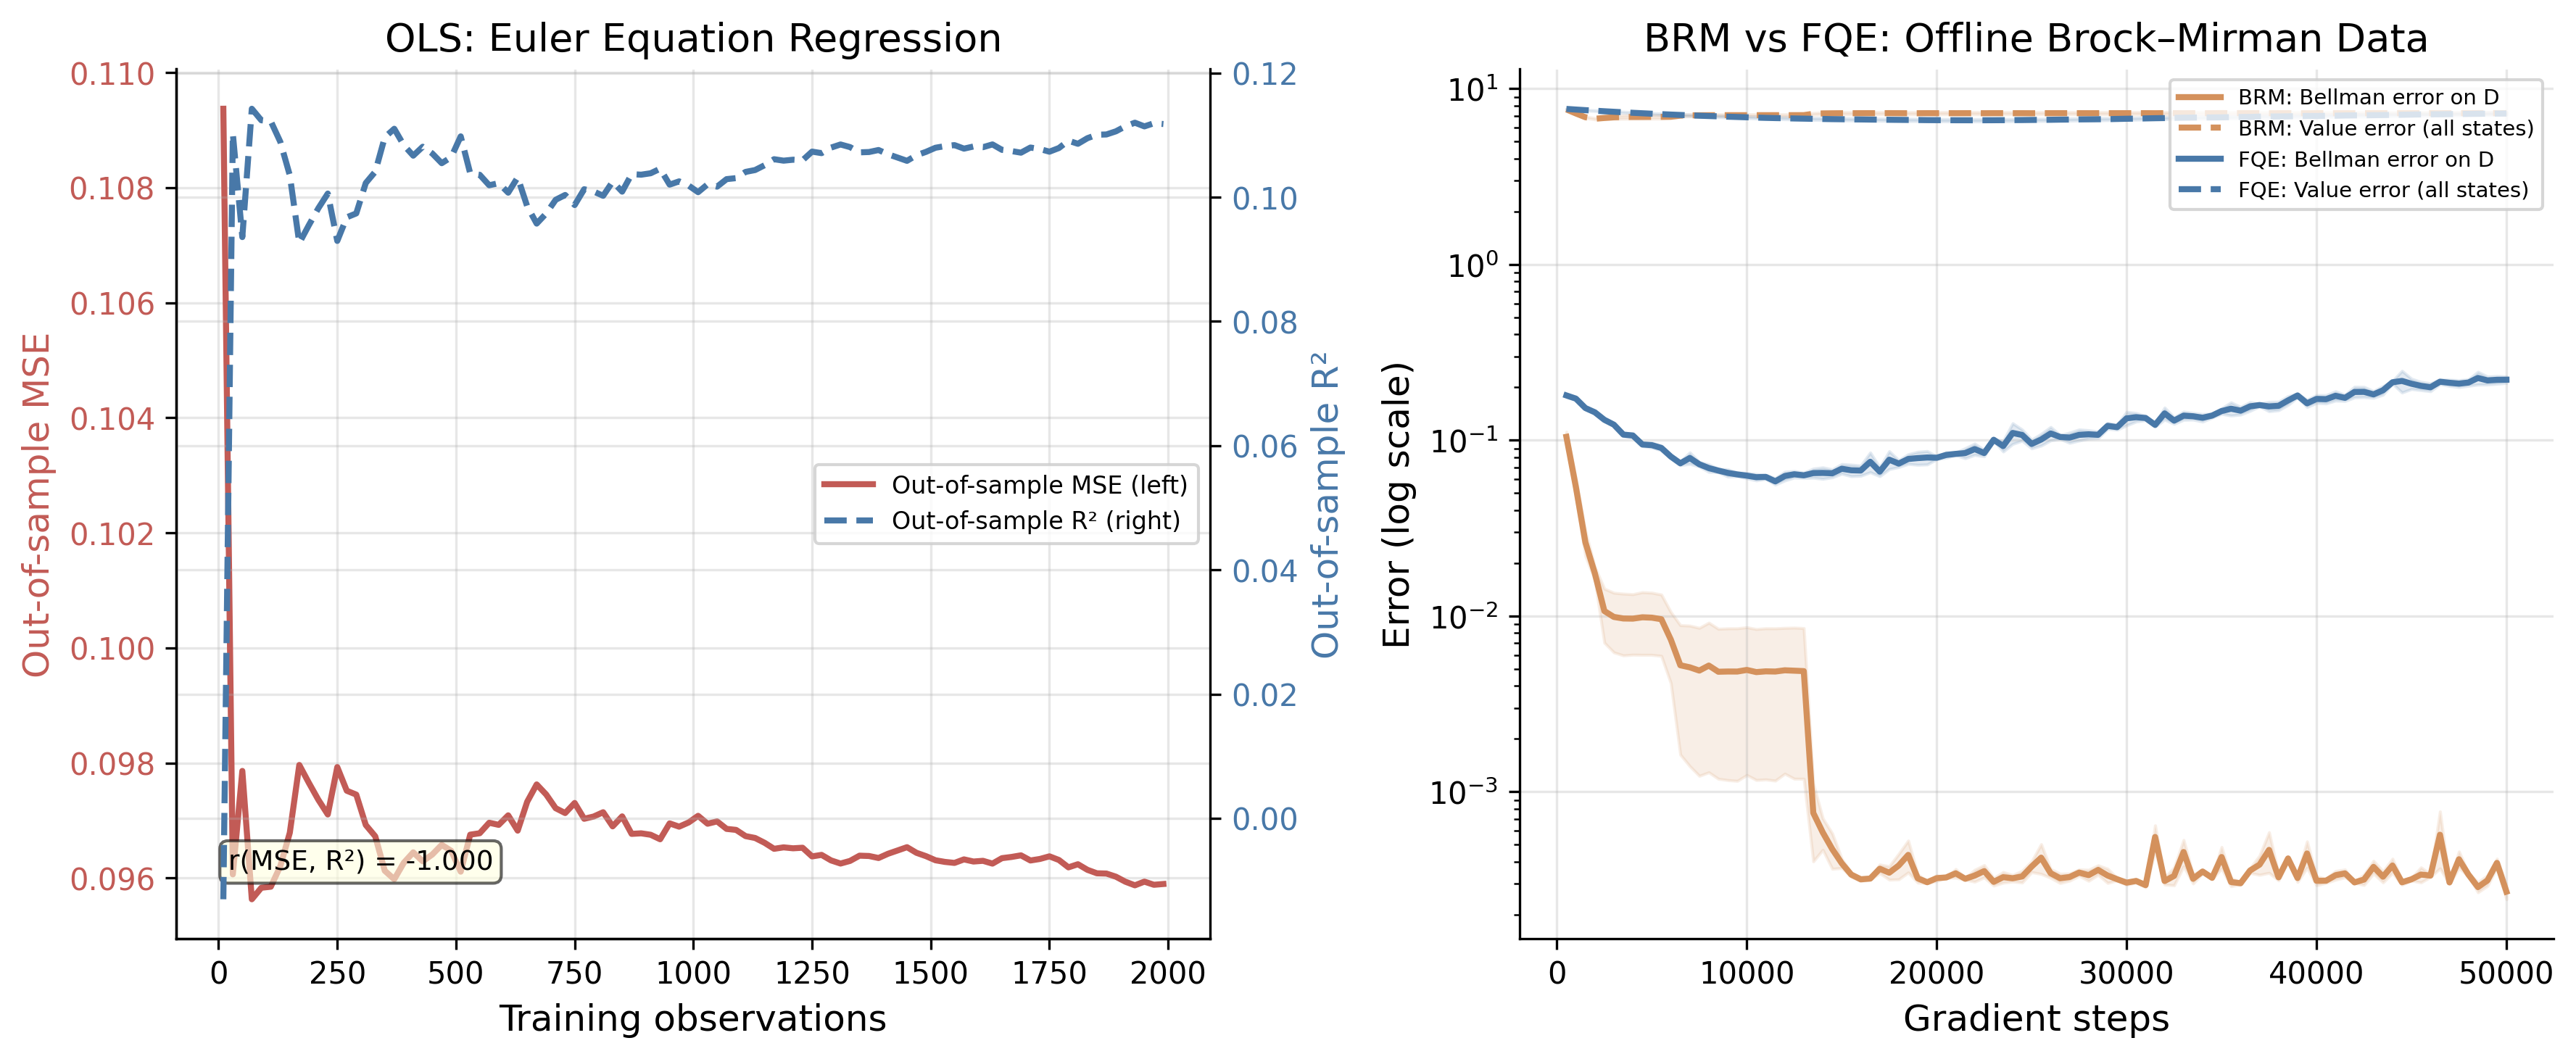
\includegraphics[width=0.9\textwidth]{../ch03b_deeprl_practice/sims/brock_mirman_bellman.png}
\caption{Left: OLS regression of log consumption on log capital and log productivity, estimated on expanding windows from the Brock--Mirman optimal policy. Out-of-sample MSE (left axis, red) and out-of-sample $R^2$ (right axis, blue) track each other with Pearson $r = -1.000$. Right: BRM (orange) and FQE (blue) trained on offline Brock--Mirman data $\mathcal{D}$ ($T = 2{,}000$ transitions, 0.2\% state-space coverage); note the log scale on the $y$-axis. Solid lines show Bellman error on $\mathcal{D}$ (current network both sides); dashed lines show mean absolute value error against $Q^*$ over all 4,795 feasible state-action pairs; shaded bands are $\pm 1$ SE over 10 seeds.}
\label{fig:bellman_vs_return}
\end{figure}

\subsection{Discussion and Recommendations}
\label{sec:checklist}

Track episode return and policy entropy alongside training loss; entropy collapse and stagnating return are early warning signs of plasticity loss (Section~\ref{sec:plasticity}). Use PPO or SAC as default baselines before implementing custom algorithms. Report at least 10 seeds per configuration with IQM-based comparisons (Section~\ref{sec:reproducibility}).

